\section*{Теория}

\subsection*{Плазменные колебания}

\begin{wrapfigure}{left}{0.5\textwidth}
	\vspace{-10pt}
	\centering
	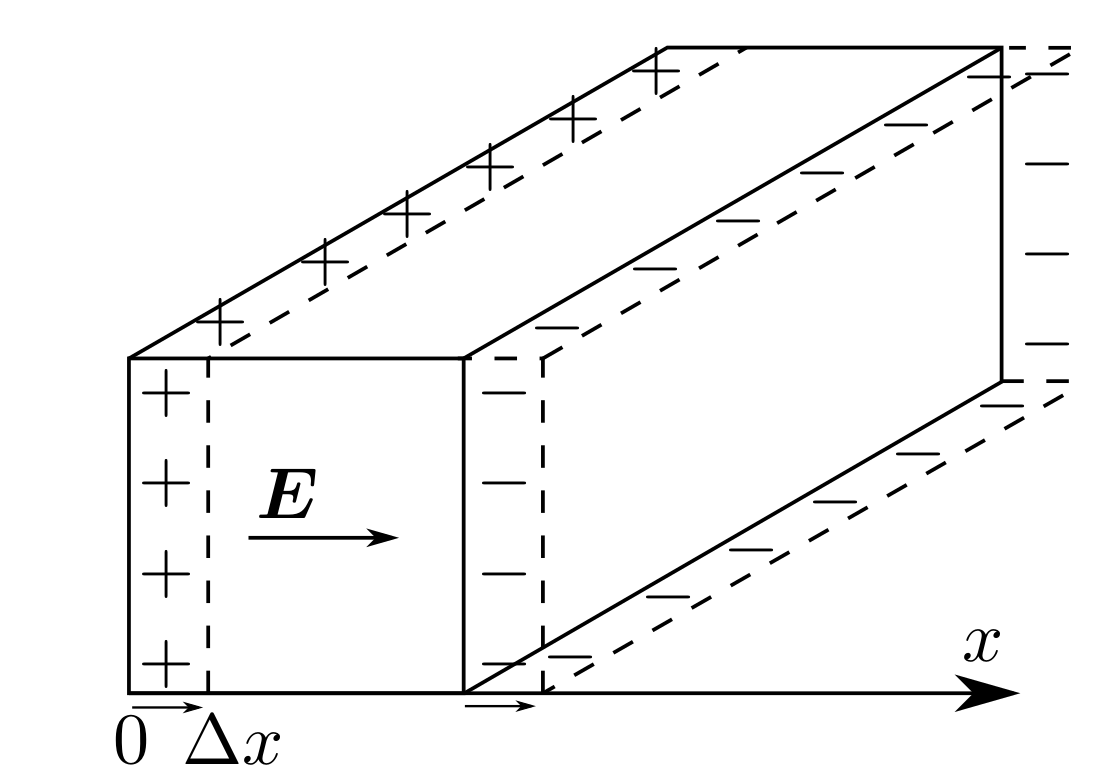
\includegraphics[width=0.48\textwidth]{../res/plasma.png}
	\caption{Плазменные колебания.}
	\label{img:plasma oscil}
\end{wrapfigure}

Выделим в нейтральной плазме некоторый объём в виде параллелепипеда. Обозначим концентрацию электронов как $n_e$; ионы для простоты будем считать однозарядными ($Z = 1$), тогда их концентрация такая же, как у электронов: $n_i = n_e$. Предположим, что все электроны сместились на расстояние $\chi$ относительно ионов. Ионы как существенно более тяжёлые частицы можно считать неподвижными. В результате на боковых гранях параллелепипеда возникнут нескомпенсированные поверхностные заряды с плотностью:
$$
\sigma = \pm n_e e \Delta x
$$
Эти заряды --- как две пластины конденсатора --- создадут электрическое поле:
$$
E = 4 \pi n_e e \Delta x
$$
В свою очередь это поле будет действовать на электроны, придавая им
ускорение, равное:
$$
\frac{d^2 \Delta x}{d t^2} = - \frac{eE}{m} = -\frac{4 \pi n_e e^2}{m} \Delta x
$$
Видно, что полученное уравнение описывает гармонические колебания
с частотой:
$$
\omega_p = \sqrt{\frac{4 \pi n_e e^2}{m_e}}
$$
Таким образом, мы получили частоту коллективных колебаний электронов относительно квазинейтрального состояния. Такие колебания называют \textit{ленгмюровскими}, а частоту $\omega_p$ -- \textit{плазменной} или \textit{ленгмюровской}. Эта частота -- один из важнейших параметров плазмы. Она определяет характерный временной масштаб для плазмы — время отклика на флуктуацию плотности заряда в ней. Частота $\omega_p$ определяет многие физические процессы, включая распространение электромагнитных волн в плазме.

\subsection*{Дебаевский радиус}

Плазменные колебания могут быть возбуждены как за счёт внешнего воздействия (например, при прохождении электромагнитной волны), так и за счёт тепловой энергии, содержащейся непосредственно в плазме. Оценим амплитуду колебаний в последнем случае. Средняя скорость теплового движения электронов по порядку величины равна $\bar v_e \sim \sqrt{\frac{k T_e}{m_e}}$, где $T_e$ - температура электронов. Амплитуду $r$ колебаний электронов относительно ионов оценим как смещение с тепловой скоростью $\bar v_e$ за характерное время плазменных колебаний $\frac{1}{\omega_p}: r = \frac{\bar v_e}{\omega_p}$. Полученную величину обозначают как
$$
r_D = \sqrt{\frac{k T_e}{4 \pi n_e e^2}} \sim \frac{\bar v_e}{\omega_p}
$$
и называют \textit{дебаевским радиусом} (или \textit{дебаевской длиной}). Это --- ещё один важный плазменный параметр, задающий характерный пространственный масштаб многих плазменных явлений.

